\section{曲线运动}

\section{小船过河}

\begin{proset}
	小明同学要过一条\,\qty{60}{m}宽、河岸平直的小河，所乘小船在静水中划行速率为\,\qty{3}{m/s}，河水流速为\,\qty{5}{m/s}，下列判断正确的是\paren[]

	\begin{choices}
		\item 过河最短时间为\,\qty{12}{s}
		\item 过河最短时间为\,\qty{20}{s}
		\item 过河最短位移为\,\qty{60}{m}
		\item 过河最短位移为\,\qty{80}{m}
	\end{choices}
\end{proset}
\begin{answer}
	B\quad 提示：最短位移\,\qty{100}{m}
	
	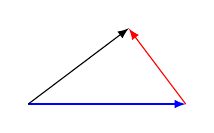
\begin{tikzpicture}[font=\scriptsize,>=latex]
		\draw[->,blue] (0,0)--(2,0);
		\draw[->,red] (2,0)--++(127:1.2);
		\draw[->] (0,0)--(37:1.6);
	\end{tikzpicture}
\end{answer}

\subsection{平抛运动}

\begin{proset}
	（多选）
    如图所示，在固定的倾角为\,\qty{37}{\degree}的斜面顶点\(A\)处，以速度\(v_0\)垂直于斜面抛出一个小球，小球落在斜面上的\(C\)点（\(C\)点未画出）反弹一次后落在斜面底端\(B\)点，反弹前后垂直于斜面的速度大小不变，沿斜面方向的速度不变。已知重力加速度大小为\(g\)，\(\sin\) \,\qty{37}{\degree}\( =0.6\)，\(\cos\) \,\qty{37}{\degree}\( = 0.8\)，不计空气阻力，下列说法正确的是\paren[]

    \begin{tikzpicture}[font=\scriptsize]
		\def\TheTa{37}%旋转角度
		\def\LenGth{4}%斜面长度
		\pgfmathsetmacro\CosLenGth{\LenGth*cos(\TheTa)}
		\begin{scope}[rotate=\TheTa]	
			\draw (0,0)node[above left]{\(B\)}--++(\LenGth,0)coordinate(a)--++(-127:{\LenGth*sin(\TheTa)});
		\end{scope}
        \draw[-latex,red] (a)node[right,black]{\(A\)}--++(127:1.2)node[rotate=37,right]{\(v_0\)};
        \shade[ball color=gray] ($(a)+(127:.08)$) circle(.08);
		\draw (.4,0) arc(0:\TheTa:.4);
		\node at(.65,.18){\,\qty{37}{\degree}};
		\foreach \x in{-.5,-.3,...,\CosLenGth}
			\draw[gray] (\x,-.2)--++(.2,.2);
		\draw[thick] (-.5,0)--({\CosLenGth+.4},0);
	\end{tikzpicture}
    \begin{choices}
        \item 小球从\(A\)点到\(C\)点与\(C\)点到\(B\)点的运动时间相等
        \item 小球落至\(B\)点与\(C\)点的速度方向相同
        \item \(A\)、\(B\)两点的距离为\(\frac{15v_0^2}{2g}\)
        \item 小球落至\(B\)点的速度大小为\(\sqrt{10}v_0\)
    \end{choices}
\end{proset}
\begin{answer}
	ACD\quad 提示：建立如图所示坐标系，\(x\)方向初速度为0的匀加速运动，\(y\)方向类上抛运动

	\begin{tikzpicture}[font=\scriptsize]
		\def\TheTa{37}%旋转角度
		\def\LenGth{4}%斜面长度
		\pgfmathsetmacro\CosLenGth{\LenGth*cos(\TheTa)}
		\begin{scope}[rotate=\TheTa]	
			\draw (0,0)node[above left]{\(B\)}--++(\LenGth,0)coordinate(a)--++(-127:{\LenGth*sin(\TheTa)});
		\end{scope}
		\draw[-latex,blue] ($(a)+(-53:1)$)--($(a)+(127:2)$)node[rotate=37,right]{\(y\)};
		\draw[-latex,blue] ($(a)+(37:.5)$)--++(-143:5)node[below,rotate=37]{\(x\)};
		\draw[-latex,red] (a)--++(0,-1)node[below right]{\(mg\)}coordinate(g);
		\draw[-latex,red] (a)--++(-53:.8)coordinate(gy);
		\draw[-latex,red] (a)--++(-143:.6)coordinate(gx);
		\draw[dashed] (gy)--(g)--(gx);
        \draw[-latex,red] (a)node[right,black]{\(A\)}--++(127:.6)node[rotate=37,right]{\(v_0\)};
		\draw (.4,0) arc(0:\TheTa:.4);
		\node at(.65,.18){\,\qty{37}{\degree}};
		\foreach \x in{-.5,-.3,...,\CosLenGth}
			\draw[gray] (\x,-.2)--++(.2,.2);
		\draw[thick] (-.5,0)--({\CosLenGth+.4},0);
	\end{tikzpicture}
\end{answer}